% #############################################################################
% This is Appendix A
% !TEX root = ../main.tex
% #############################################################################
\chapter{On Bessel Functions}\label{appendix_c_bessel}

In this Appendix, some theory regarding Bessel functions is presented since they naturally appear when studying the Laplace operator, in the fundamental solution of the Helmholtz equation, when solving it in polar coordinates, and they are essential in the proof of Proposition \ref{dirac_not_polar}. First, some of its properties and relations are stated. Then, a short proof of the fundamental solution of the Helmholtz equation is given. Most of this Appendix is based on the classical book \cite{abramowitz1988handbook} and \cite{chen2010boundary}.

Let \(\nu \in \mathbb{C}\). Bessel functions are the solutions \(y(x)\) of the differential equation
\begin{equation}\label{bessel_equation}
    x^2\frac{\partial^2 y}{\partial x^2} + x \frac{\partial y}{\partial x} + (x^2-\nu^2)y = 0.
\end{equation}

Since equation \eqref{bessel_equation} is a second-order linear differential equation, its two linearly independent solutions are the Bessel functions of first kind and second kind, \(J_\nu\) and \(Y_\nu\), respectively. The Bessel function of first kind can be represented by the series
\[
    J_\nu (z) = \left(\frac{1}{2}z\right)^\nu \sum_{k=0}^{\infty} \frac{\left(-\frac{1}{4}z^2\right)^k}{k! \Gamma(\nu+k+1)},
\]
where \(\Gamma(z) = \int_0^\infty t^{z-1} e^{-t}dt\) is the special Gamma function. For the Bessel function of second kind, series expansions are only available for \(\nu \in \mathbb{N}\). However, the relation \eqref{bessel_y_relation} holds
\begin{equation}\label{bessel_y_relation}
    Y_\nu(z) = \frac{J_\nu(z) \cos(\nu \pi) - J_{-\nu}(z)}{\sin(\nu \pi)}.
\end{equation}

Both functions are holomorphic through the complex plane cut along the negative real axis. If \(\nu \in \mathbb{N}\), then \(J_\nu\) is an entire function, i.e., holomorphic in the whole complex plane. In any other cases, both Bessel functions display a singularity on the origin: if \(\nu > 0\) then \(J_\nu(0)=0\), but it is not differentiable at the origin; for any other cases \(J_\nu(0)\) and \(Y_\nu(0)\) do not exist. Figures \ref{bessel_function_j_complex_plot} and \ref{bessel_function_y_complex_plot} present the Bessel functions of first and second kinds. The plots were created using Wolfram Mathematica.

\begin{figure}[!htb]
    \centering
    \begin{minipage}{.5\textwidth}
        \centering
        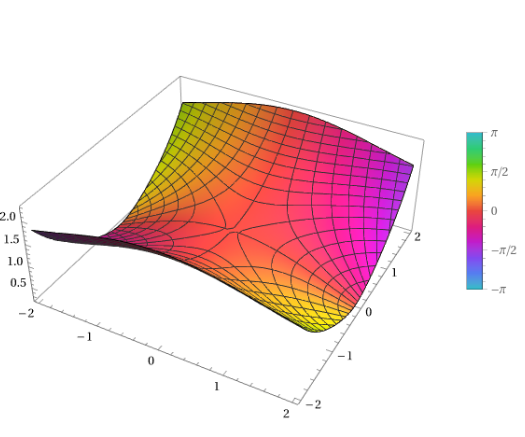
\includegraphics[width=\linewidth]{Images/Bessel/bessel_j_0_z.png}
        \captionsetup{width=0.9\linewidth} % Adjust the width of the caption
        \caption{Plot of the Bessel function \(J_\nu(z)\) with \(\nu=0\) in the complex plane from \(-2-2i\) to \(2+2i\).}
        \label{bessel_function_j_complex_plot}
    \end{minipage}%
    %\hspace{0.2cm} % Add some horizontal space between the figures
    \begin{minipage}{.5\textwidth}
        \centering
        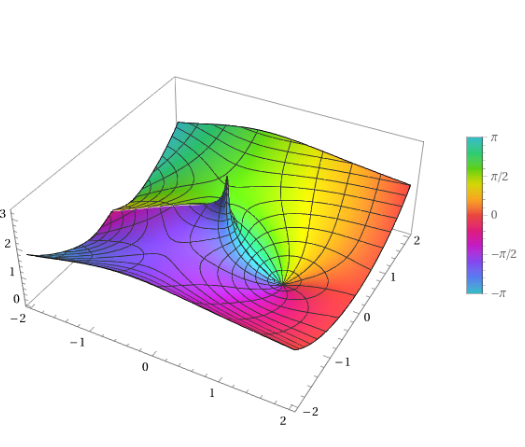
\includegraphics[width=\linewidth]{Images/Bessel/bessel_y_0_z.png}
        \captionsetup{width=0.9\linewidth} % Adjust the width of the caption
        \caption{Plot of the Bessel function \(Y_\nu(z)\) with \(\nu_=0\) in the complex plane from \(-2-2i\) to \(2+2i\).}
        \label{bessel_function_y_complex_plot}
    \end{minipage}
\end{figure}

A particularly important Bessel function in this work was the Bessel functions of third kind, known as Hankel functions \(H_\nu^{(1)}(z), H_\nu^{(2)}(z)\). Those functions are also known as the Hankel function of first and second kind, respectively, and are defined using the \(J_\nu(z)\) and \(Y_\nu(z)\) Bessel functions:
\begin{align*}
    &H_\nu^{(1)}(z) = J_\nu(z) + i Y_\nu(z)\\
    &H_\nu^{(2)}(z) = J_\nu(z) - i Y_\nu(z),
\end{align*}
and therefore also satisfy equation \eqref{bessel_equation}.

Figures \ref{hankel_function_1_complex_plot} and \ref{hankel_function_2_complex_plot} present the Hankel functions of first and second kinds and Proposition \ref{asympt_hankel_app_c} presents the asymptotic expansions for small and large arguments of \(H_\nu^{(1)}(z)\) and \(H_\nu^{(2)}(z)\).

\begin{figure}[H]
    \centering
    \begin{minipage}{.5\textwidth}
        \centering
        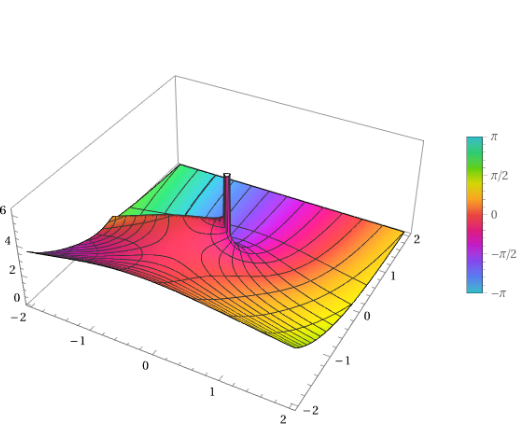
\includegraphics[width=\linewidth]{Images/Bessel/hankel_1_0_z.png}
        \captionsetup{width=0.9\linewidth} % Adjust the width of the caption
        \caption{Plot of the Hankel function \(H_\nu^{(1)}(z)\) with \(\nu=0\) in the complex plane from \(-2-2i\) to \(2+2i\).}
        \label{hankel_function_1_complex_plot}
    \end{minipage}%
    %\hspace{0.2cm} % Add some horizontal space between the figures
    \begin{minipage}{.5\textwidth}
        \centering
        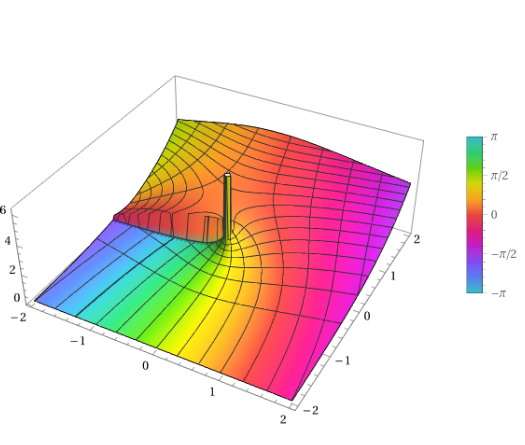
\includegraphics[width=\linewidth]{Images/Bessel/hankel_2_0_z.png}
        \captionsetup{width=0.9\linewidth} % Adjust the width of the caption
        \caption{Plot of the Hankel function \(H_\nu^{(2)}(z)\) with \(\nu_=0\) in the complex plane from \(-2-2i\) to \(2+2i\).}
        \label{hankel_function_2_complex_plot}
    \end{minipage}
\end{figure}

\begin{proposition}\label{asympt_hankel_app_c}
    Let \(\nu \in \mathbb{C}\). The limiting forms of the Hankel functions \(H_0^{(1)}(z)\) and \(H_0^{(2)}(z)\) for a small argument \(z\) take the form,
    \begin{align*}
        &H_\nu^{(1)}(z) \sim
        \begin{cases}
            -\frac{2 \pi}{i} \log z, & \nu = 0\\
            \frac{1}{i \pi} \Gamma(\nu) \left(\frac{1}{2}z\right)^{-\nu}, & \nu \neq 0
        \end{cases}
    \end{align*}
    and
    \begin{align*}
        &H_\nu^{(2)}(z) \sim 
        \begin{cases}
            \frac{2 \pi}{i} \log z, & \nu = 0\\
            -\frac{1}{i \pi} \Gamma(\nu) \left(\frac{1}{2}z\right)^{-\nu}, & \nu \neq 0,
        \end{cases}
    \end{align*}
    when \(z \rightarrow 0\) and \(\Re{\nu} \geq 0\). On the other hand, the asymptotic expansions for large arguments are 
    \begin{align*}
        &H_\nu^{(1)}(z) \sim \sqrt{\frac{2}{\pi z}}e^{i\left(z-\frac{1}{2}\nu \pi - \frac{1}{4}\pi\right)}, \text{ if } -\pi < \arg z < 2 \pi\\
        &H_\nu^{(2)}(z) \sim \sqrt{\frac{2}{\pi z}}e^{-i\left(z-\frac{1}{2}\nu \pi - \frac{1}{4}\pi\right)}, \text{ if } -2\pi < \arg z < \pi
    \end{align*}
    when \(\abs{z} \rightarrow \infty\).
\end{proposition}

Before presenting the proof of the Helmholtz equation's fundamental solution, some recurrence relations are stated, which were used in the proof of Proposition \ref{dirac_not_polar}.

\begin{proposition}\label{recurrence_bessel_appendix_c}
    Let \(\mathcal{Z}_\nu\) denote \(J_\nu, Y_\nu, H^{(1)}_\nu\) or \(H^{(2)}_\nu\) for any \(\nu \in \mathbb{C}\). The following recurrence relations hold:
    \begin{align*}
        &\mathcal{Z}_{\nu-1}(z) + \mathcal{Z}_{\nu+1}(z) = \frac{2 \nu}{z}\mathcal{Z}_{\nu}(z)\\
        &\mathcal{Z}_{\nu-1}(z) - \mathcal{Z}_{\nu+1}(z) = 2\frac{d \mathcal{Z}_{\nu}(z)}{dz}\\
        &\frac{d \mathcal{Z}_{\nu}(z)}{dz} = \mathcal{Z}_{\nu-1}(z) - \frac{\nu}{z}\mathcal{Z}_{\nu}(z) \\
        &\frac{d \mathcal{Z}_{\nu}(z)}{dz} = -\mathcal{Z}_{\nu+1}(z) + \frac{\nu}{z}\mathcal{Z}_{\nu}(z).
    \end{align*}
    In particular,
    \[
        \frac{d \mathcal{Z}_{0}(z)}{dz} = -\mathcal{Z}_{1}(z).
    \]
\end{proposition}

Let \(k \in \mathbb{C}\) such that \(\Im{k} \geq 0\) and \(\Phi_k(x)\) be the fundamental solution of the Helmholtz equation, i.e.,

\begin{equation}\label{appendix_c_invariant}
    -\left(\Delta \Phi_k(x) + k^2 \Phi_k(x)\right) = \delta_0(x).
\end{equation}

First, one proves that equation \eqref{appendix_c_invariant} is invariant under rotations.

\begin{lemma}\label{invariant_lemma}
    Let \(\Phi_k(x)\) be a solution of equation \eqref{appendix_c_invariant}. Then, \(\Phi_k(R x)\) is also a solution, where \(R\) is a rotation (orthogonal) matrix, such that \(R^T = R^{-1}\).
\end{lemma}
\begin{proof}
    The proof is straightforward and only uses the chain rule. Let \(\psi(x) = \Phi_k(Rx)\). Then,
    \begin{align*}
        &\nabla \psi(x) = R^T \nabla \Phi_k(R x)\\
        &\Delta \psi(x) = R^T R \Delta \Phi_k(R x) = \Delta \Phi_k(R x)
    \end{align*}
    by the orthogonality property of matrix \(R\). Since \(R\) is a bijective map from \(\mathbb{R}^2\) to \(\mathbb{R}^2\), the claim follows.
\end{proof}

\begin{proposition}
    The function \(\Phi_k: \mathbb{R}^d \setminus \{0\} \rightarrow \mathbb{R}\) given by
    \[
    \Phi_k(x) = \begin{cases}
        \frac{i}{4} H_0^{(1)}(k \norm*{x}), & d=2\\
        \frac{e^{i k \norm*{x}}}{4 \pi \norm*{x}}, & d = 3
    \end{cases}    
    \]
    is the fundamental solution of the Helmholtz equation \eqref{appendix_c_invariant}.
\end{proposition}
\begin{proof}
    Let \(x \in \mathbb{R}^d \setminus \{0\}\) and \(\Phi_k\) be the solution of
    \begin{equation}\label{proof_fs_helm_appendix_c}
        \Delta \Phi_k(x) + k^2 \Phi_k(x) = 0.
    \end{equation}
    Considering equation \eqref{proof_fs_helm_appendix_c} in polar coordinates, by Lemma \ref{invariant_lemma} it suffices to consider the radial part of equation
    \[
        \frac{1}{r^{d-1}} \frac{d}{d r}\left(r^{d-1}\frac{d \Phi_k(r)}{d r}\right) + k^2\Phi_k(r) = 0 \iff \frac{d}{d r}\left(r^{d-1}\frac{d \Phi_k(r)}{d r}\right) + k^2 r^{d-1}\Phi_k(r) = 0.
    \]
    Through the change of variables \(\Phi_k(r) = r^{1-\frac{d}{2}}\psi(r)\), the equation above can be written as
    \[
        \frac{d}{d r}\left(r \frac{d \psi(r)}{d r}\right) + \left(k^2 r - \frac{\left(\frac{1}{2}d-1\right)^2}{r}\right)\psi(r) = 0,
    \]
    and after differentiating the first term and multiplying by \(r\) one finds that 
    \[
        r^2\frac{d^2 \psi(r)}{d r^2} + r\frac{d \psi(r)}{d r} + \left(\left(kr\right)^2-\left(\frac{1}{2}d-1\right)^2\right) = 0.
    \]
    Making another change of variables \(\rho = k r\) one obtains the equation \eqref{bessel_equation}
    \[
        \rho^2\frac{d^2 \psi(\rho)}{d \rho^2} + \rho\frac{d \psi(\rho)}{d \rho} + \left(\rho^2-\left(\frac{1}{2}d-1\right)^2\right) = 0,
    \] 
    whose solution (in the complex numbers) is given by the Hankel functions (or order \(\frac{1}{2}d-1\))
    \[
        \psi(\rho) = A H^{(1)}_{\frac{1}{2}d-1}(\rho) + B H^{(2)}_{\frac{1}{2}d-1}(\rho),
    \]
    where \(A, B \in \mathbb{C}\) and 
    \[
        \Phi_k(r) = r^{1-\frac{d}{2}} \left(A H^{(1)}_{\frac{1}{2}d-1}(kr) + B H^{(2)}_{\frac{1}{2}d-1}(kr)\right).
    \]
    Since \(\Phi_k\) must satisfy the \ref{sommerfeld_conditions} and \(\Im{k} \geq 0\) it implies that \(B=0\) by Proposition \ref{asympt_hankel_app_c} and
    \[
        \Phi_k(r) = r^{1-\frac{d}{2}} A H^{(1)}_{\frac{1}{2}d-1}(kr).
    \]
    To find \(A\), one can integrate on the ball \(B_\epsilon(0)\), apply the Divergence Theorem \ref{appendix_div_theor} and by Proposition \ref{asympt_hankel_app_c}
    \[
        \int_{\partial B_\epsilon(0)} \frac{\partial \Phi_k(r)}{\partial n}d \sigma \rightarrow -1, \, \epsilon \rightarrow 0.
    \] 
    On the other hand
    \[
        \int_{\partial B_\epsilon(0)} \frac{\partial \Phi_k}{\partial n}d \sigma = \abs{\partial B_1(0)} \epsilon^{d-1}\Phi_k'(\epsilon)
    \]
    which implies that
    \[
        \abs{\partial B_1(0)} \epsilon^{d-1}\Phi_k'(\epsilon) \rightarrow -1, \, \epsilon \rightarrow 0.
    \]
    From the formulas in Proposition \ref{recurrence_bessel_appendix_c} the equation above can be written as
    \[
        -A k  \abs{\partial B_1(0)} \epsilon^{\frac{d}{2}}H^{(1)}_{\frac{d}{2}}(k \epsilon) \rightarrow -1, \, \epsilon \rightarrow 0,
    \]
    which is asymptotically equal to
    \[
        A k \abs{\partial B_1(0)} \frac{i 2^{\frac{d}{2}} \Gamma(\frac{d}{2})}{\pi}  \rightarrow -1, \, \epsilon \rightarrow 0
    \]
    by Proposition \ref{asympt_hankel_app_c} and,
    \[
        A = \frac{i \pi 2^{-\frac{d}{2}}k^{\frac{(d-2)}{2}}}{\Gamma(\frac{d}{2})\abs{\partial B_1(0)}}.
    \]
    Since \(\abs{\partial B_1(0)} = \frac{2 \pi^{\frac{d}{2}}}{\Gamma\left(\frac{1}{2}d\right)}\), 
    and 
    \[
        H^{(1)}_{\frac{1}{2}}(z) = \frac{1}{i}\sqrt{\frac{2}{\pi}}\frac{e^{i z}}{\sqrt{z}}
    \]
    for \(d=3\), the fundamental solution of the Helmholtz equations is given by
    \[
        \Phi_k(r) = \begin{cases}
            \frac{i}{4} H_0^{(1)}(k r), & d=2\\
            \frac{e^{i k r}}{4 \pi r}, & d = 3.
        \end{cases}    
    \]
\end{proof}

Figures \ref{hankel_function_re} and \ref{hankel_function_im} present the real and imaginary part of the fundamental solution \(\frac{i}{4} H_0^{(1)}(k r)\), respectively.

\begin{figure}[H]
    \centering
    \begin{minipage}{.5\textwidth}
        \centering
        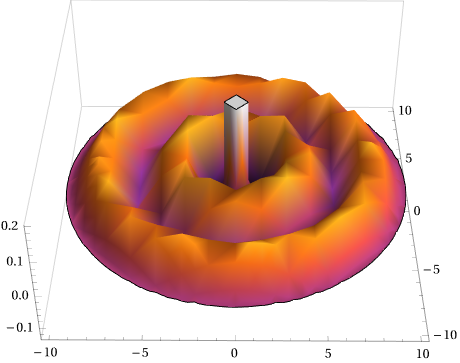
\includegraphics[width=\linewidth]{Images/Bessel/hankel_re.png}
        \captionsetup{width=0.9\linewidth} % Adjust the width of the caption
        \caption{Plot of the real part of \(\Phi_k(r)\) with \(k=1.5\) in the disk of radius \(10\).}
        \label{hankel_function_re}
    \end{minipage}%
    %\hspace{0.2cm} % Add some horizontal space between the figures
    \begin{minipage}{.5\textwidth}
        \centering
        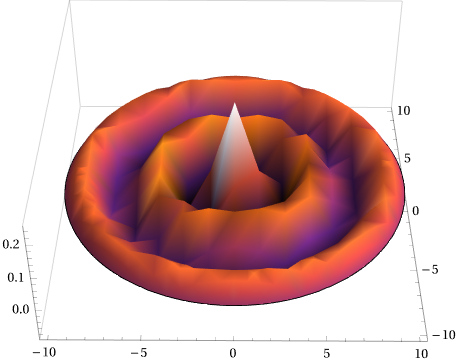
\includegraphics[width=\linewidth]{Images/Bessel/hankel_im.png}
        \captionsetup{width=0.9\linewidth} % Adjust the width of the caption
        \caption{Plot of the imaginary part of \(\Phi_k(r)\) with \(k=1.5\) in the disk of radius \(10\).}
        \label{hankel_function_im}
    \end{minipage}
\end{figure}